To better illustrate the optimization potential of opportunistic evaluation, we present two typical data analysis scenarios that could benefit from asynchronous execution of queries during \thinktime to minimize interactive latency. 
While the user's program remains the same, we illustrate the modifications to the execution plan that highlights the transformations made. 


\subsubsection{Interaction-based Reordering}
Consider a common workflow of analyzing multiple data files, shown on the left in Figure~\ref{fig:files}.
The user, Sam, executes the first cell, which loads both of the files, and is forced to wait for \emph{both} to finish loading before she can interact with \emph{either} of the dataframes. 
To reduce the interactive latency (as perceived by the user), we could conceptually re-order the code to optimize for the immediate output.  As shown on the right in Figure~\ref{fig:files}, the re-ordered program defers loading the large file to after the interaction, \code{df1.describe()}, obviating the need to wait for the large file to load into \code{df2} before Sam can start inspecting the content of the small file.
To further reduce the interactive latency, the system could load \code{df2} while Sam is viewing the results of \code{df1.describe()}. This way, the time-consuming process of loading the large file is completed during Sam's \thinktime, thus reducing the latency for interacting with \code{df2}.

\begin{figure}[h!]
    \centering
    \begin{subfigure}%{0.4\textwidth}
    %\vspace{-3pt}
         \centering
         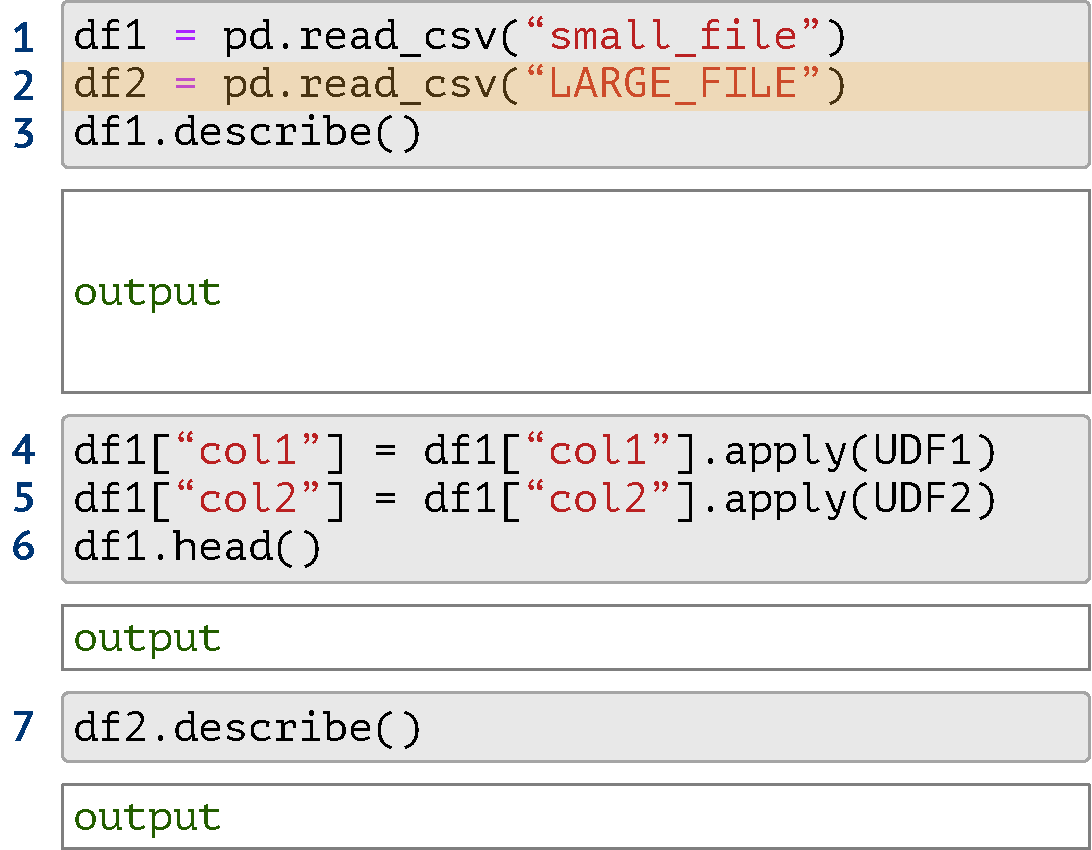
\includegraphics[width=0.4\textwidth]{submissions/interactivity/figures/reorderOrig.pdf}
         %\caption{Original program where user has to wait for both files to load before viewing any.}
         %\label{fig:orig_files}
    \end{subfigure}
    \hspace{10pt}
    \begin{subfigure}%{0.44\textwidth}
         \centering
         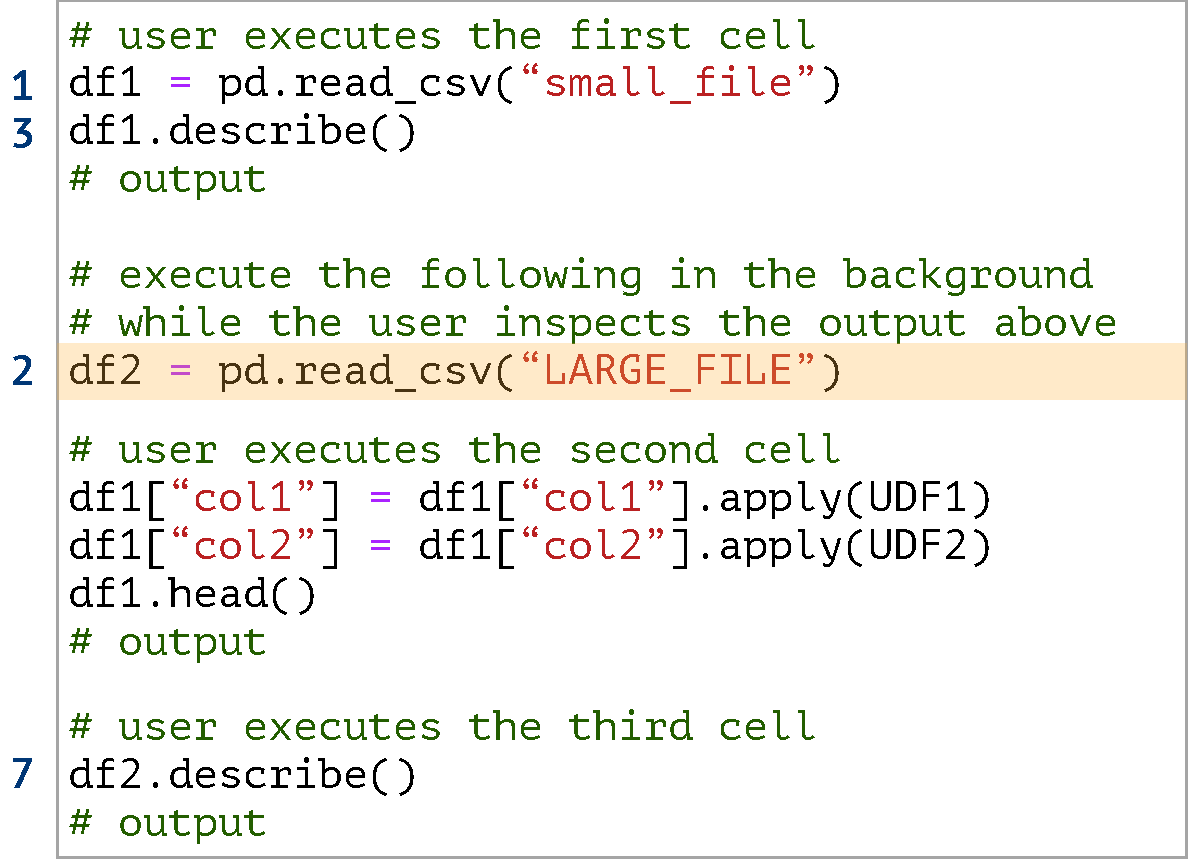
\includegraphics[width=0.44\textwidth]{submissions/interactivity/figures/reorderOpt.pdf}
         %\caption{Optimized program where the user can view the smaller file first while the other loads.}
         %\label{fig:opt_files}
    \end{subfigure}
    %\vspace{-8pt}
    \caption{Example program transformation involving operator reordering: (left) Original program where user has to wait for both files to load before viewing any; (right) Optimized program where the user can view the smaller file first while the other loads.}
    \label{fig:files}
    %\vspace{-8mm}
\end{figure}

\subsubsection{Prioritizing Partial Results}
For any large dataframes, users can only inspect a handful of rows at a time.  However the current evaluation mechanism requires \emph{all} the rows to be evaluated.  Expensive queries such as those involving user-defined functions (UDFs) could take a long time to fully compute, as shown on the left in Figure~\ref{fig:partial}.

To reduce interactive latency, one can prioritize computation of only the portion of the dataframe inspected.  This method is essentially an application of \textit{predicate pushdown}, a standard technique from database query optimization.
The right part of Figure~\ref{fig:partial} provides an example transformation for the particular operator, \code{groupby}.
While the first cell prioritizes the computation of the inspected rows, the user may still need the result of the entire computation, which is scheduled to be computed later while Sam is still reading the result of the previous cell, \code{groupNow.head(10)}, i.e. the \thinktime.
A noteworthy attribute of dataframes is row and column equivalence~\cite{petersohn13towards}, which means that
predicate pushdown can also happen when projecting columns as well.

\begin{figure}[h!]
     \centering
     \begin{subfigure}%[b]{0.4\textwidth}
         \centering
         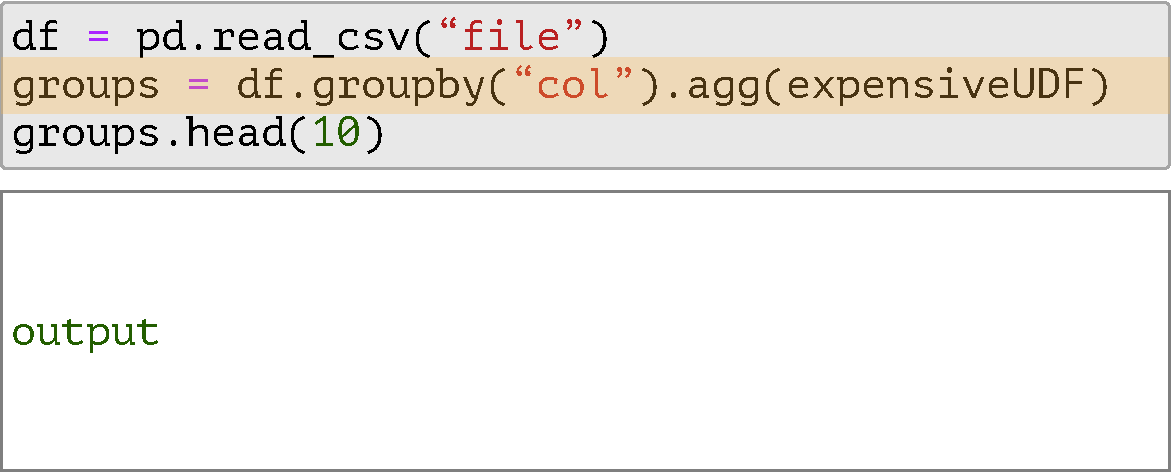
\includegraphics[width=0.4\textwidth]{submissions/interactivity/figures/predOrig.pdf}
         %\caption{Original program where the user has to wait for an expensive UDFs to fully compute.}
         %\label{fig:orig_partial}
     \end{subfigure}
     \hfill
     \begin{subfigure}%[b]{0.55\textwidth}
         \centering
         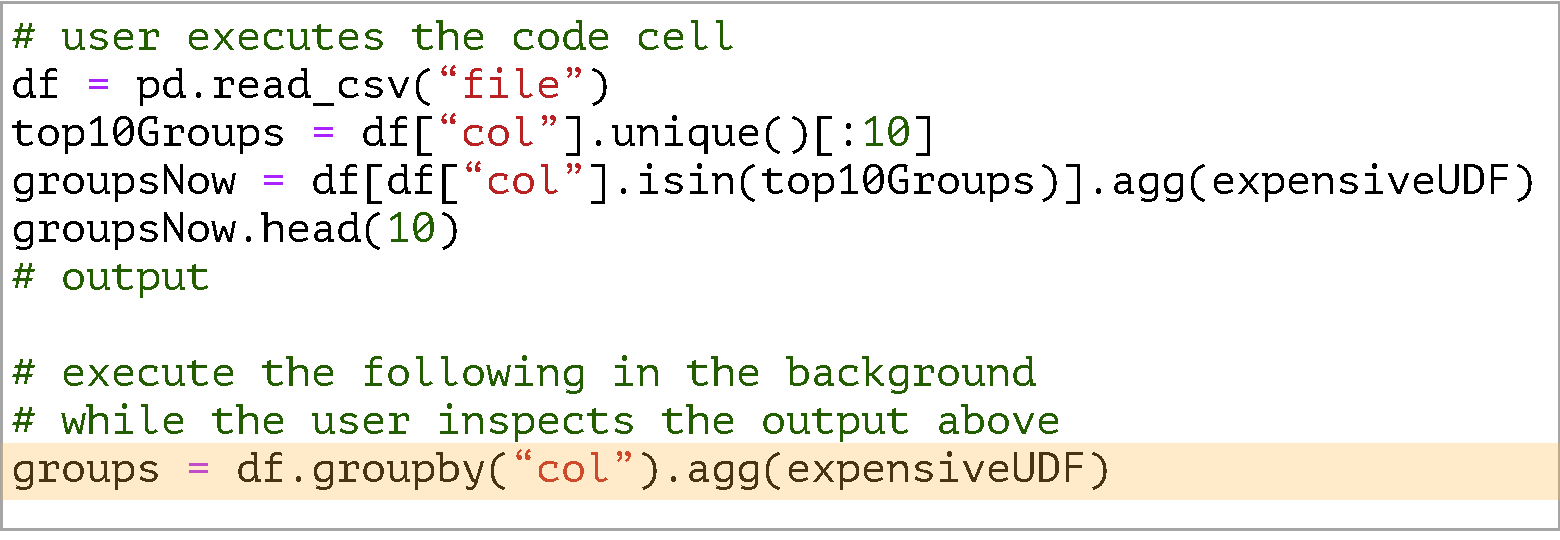
\includegraphics[width=0.55\textwidth]{submissions/interactivity/figures/predOpt.pdf}
         %\caption{Optimized program where the user can view a partial result sooner.}
         %\label{fig:opt_partial}
     \end{subfigure}
        \caption{Program transformation involving predicate pushdown. (left) Original program where the user has to wait for an expensive UDFs to fully compute; (right) Optimized program where the user can view a partial result sooner.
        }
        \label{fig:partial}
\end{figure}
